\documentclass[slidestop,compress,mathserif, aspectratio = 169]{beamer}
\usetheme{metropolis}
%\usepackage{helvet}
\useinnertheme{rectangles}\usepackage[round]{natbib}
\usepackage{bibentry}
\usepackage{graphicx}
\usepackage{epigraph}
\usepackage{makeidx}
\usepackage[]{amsmath}
\usepackage[]{amssymb}
\usepackage{color}
\usepackage{pict2e}
\usepackage{algorithm2e}
\usepackage[ngerman]{babel}
\usepackage{tikz}
\usetikzlibrary{mindmap}
\usepackage{multirow}
\usepackage[utf8]{inputenc}
\usepackage{multimedia}
\usepackage{xcolor}
\usepackage{keyval}
\usepgfmodule{shapes}
\usepackage{pgfplots}
\usepackage{sansmath}
\usepackage{pgfgantt}
\usetikzlibrary{arrows}
\usepackage{colortbl}
\usepackage{array}
\usepackage{transparent}
\usepackage{txfonts}
\usepackage{eurosym}

\graphicspath{{../../../../Vorlesungen/figures/}{./photos/}}

\makeatletter
\tikzset{
  base/.is choice,
  base/top/.code={\let\vbox\vtop},
  base/bottom/.code={\def\pgfutil@minipage[t]{\minipage[b]}},
  % base/bottom/.code={}, % for plain TeX
}
\makeatother


\definecolor{mint}{rgb}{0,172,177}

 \pgfplotsset{width=7cm, height = 7cm}



\begin{document}

\newcommand{\source}[1]{\rotatebox{90}{\tiny \color{gray} #1}}

\newcommand{\done}{${\color{teal}\checkmark}$}

%% Formalia
\title{IMechE Railway Challenge}
\subtitle{Praxisnah und ``as sexy as we can possibly get''}
\author{Raphael Pfaff}
\institute[FH Aachen]{Fachhochschule Aachen}
\logo{\put(-18, -100){\includegraphics[width=1.4cm]{logoR}}}




\usebackgroundtemplate{\includegraphics[width= \paperwidth]{Innotrans2018pale.jpg}}

\frame{\titlepage}

%\section{Fachgruppe Schienenfahrzeugtechnik}

\usebackgroundtemplate{}

{
\usebackgroundtemplate{\includegraphics[width= \paperwidth]{EmmaCastlepale.jpg}}

%\section{IMechE Railway Challenge}

\usebackgroundtemplate{}


\frame{\frametitle{Was ist die IMechE Railway Challenge?}
\framesubtitle{Die IMechE nutzt viele Kan\"ale, um junge Menschen f\"ur die Eisenbahn zu begeistern, die Railway Challenge ist einer davon.}
\begin{columns}[t] 
     \begin{column}[T]{7cm} 
     		\only<1>{
		\begin{itemize}
		\item Wettbewerb f\"ur Studierende, Azubis und Berufseinsteiger ($<$ 2 Jahre)
		\item Konstruktion und Bau einer Parkbahn-Lokomotive
		\item Relevante Disziplinen, z.B. 
		\begin{itemize}
		\item ATO-Zielbremsung
		\item Zuverl\"assigkeit
		\item L\"armreduzierung
		\item Energier\"uckgewinnung
		\item Fahrkomfort
		\item Innovation Paper
		\item Business Case
		\end{itemize}
		\end{itemize}}
		\only<2->{
		\begin{itemize}
		\item Raum f\"ur Innovation, in Aachen z.B.:
		\begin{itemize}
		\item Batteriefahrzeug:
		\begin{itemize}
		\item LTO-Hochleistungsbatterie
		\item LiFePo-Batterie hoher Kapazit\"at
		\end{itemize}
		\item IoT-Connection
		\item Robot Operating System
		\item Autonomes Fahren
		\begin{itemize}
		\item Lidar
		\item Stereokamera
		\item RTK-Lokalisierung
		\end{itemize}
		\end{itemize}
		\end{itemize}}
     	     \end{column}
     	\begin{column}[T]{7cm} 
         	\begin{center}
	%\vspace{-1cm}
            		\includegraphics[width=\textwidth]{EmmaDriver}
        		\end{center}
     \end{column}
 \end{columns}
 \vspace{.5cm}
\only<3>{ \begin{itemize}
	\item Kompletter Projektzyklus in 10 Monaten abgebildet - vom Lastenheft bis zur Abnahme
	\item Durch Skalierung (etwa 1:5) kosteng\"unstig und handhabbar
\end{itemize}}
}

\frame{\frametitle{Welchen Vorteil haben die Studierenden?}
\framesubtitle{Das Erlernte kann sofort in die Praxis eingebracht werden, es kann diskutiert, geschraubt, get\"uftelt und getestet werden. Durch die Abbildung des gesamten Lebenszyklus' ist f\"ur jeden etwas dabei!}
\begin{columns}[t] 
     \begin{column}[T]{7cm} 
     	\begin{itemize}
     		\item Praxiserfahrung
		\item Vernetzung
		\item Roter Faden durch Lehrveranstaltungen und Praktika
		\item Internationalit\"at
		\item Vertiefung ohne B\"uffeln
		\item Sich ausprobieren k\"onnen
		\item Erfolge genie{\ss}en
		\item Aus Misserfolgen lernen
		\item Spa{\ss}!
     	\end{itemize}
     \end{column}
     	\begin{column}[T]{7cm} 
         	\begin{center}
		\vspace{-.5cm}
            		\href{https://youtu.be/fHj4erGb14A}{\includegraphics[width=0.9\textwidth]{Winners2019}} \source{Klicken f\"ur Video}\\
			Emma $\heartsuit$ J.I.M. \\
			Grand Champion \\
			IMechE Railway Challenge 2019
        		\end{center}
     \end{column}
 \end{columns}
}

%\frame{\frametitle{Sponsoring f\"ur Emma und das Team}
%\framesubtitle{}
%         	\begin{center}
%            		
\includegraphics[width=\textwidth]{Sponsoren2019}\source{}
%        		\end{center}
%  }

%\frame{\frametitle{Was Emma braucht, um erfolgreich zu sein...}
%\framesubtitle{}
%\begin{columns}[t] 
%     \begin{column}[T]{6cm} 
%     	\begin{itemize}
%     		\item<1-> Motivierte Studis
%		\item<2-> Viel Liebe
%		\item<3-> Leere Bierkisten
%		\item<4-> Viel mehr Probefahrten
%		\only<5->{\item Hardware, insbesondere:
%		\begin{itemize}
%		\item Camera und Laserscanner
%		\item Kompakte Batterien
%		\item Federspeicherbremsen
%		\item Kompressor
%		\item 4G/WiFi Connection
%		\item Sandungssystem
%		\end{itemize}
%		}
%     	\end{itemize}
%	%\only<6>{2019 mit Ihnen als Sponsor?}
%     \end{column}
%     	\begin{column}[T]{8cm} 
%         	\begin{center}
%            		\only<1>{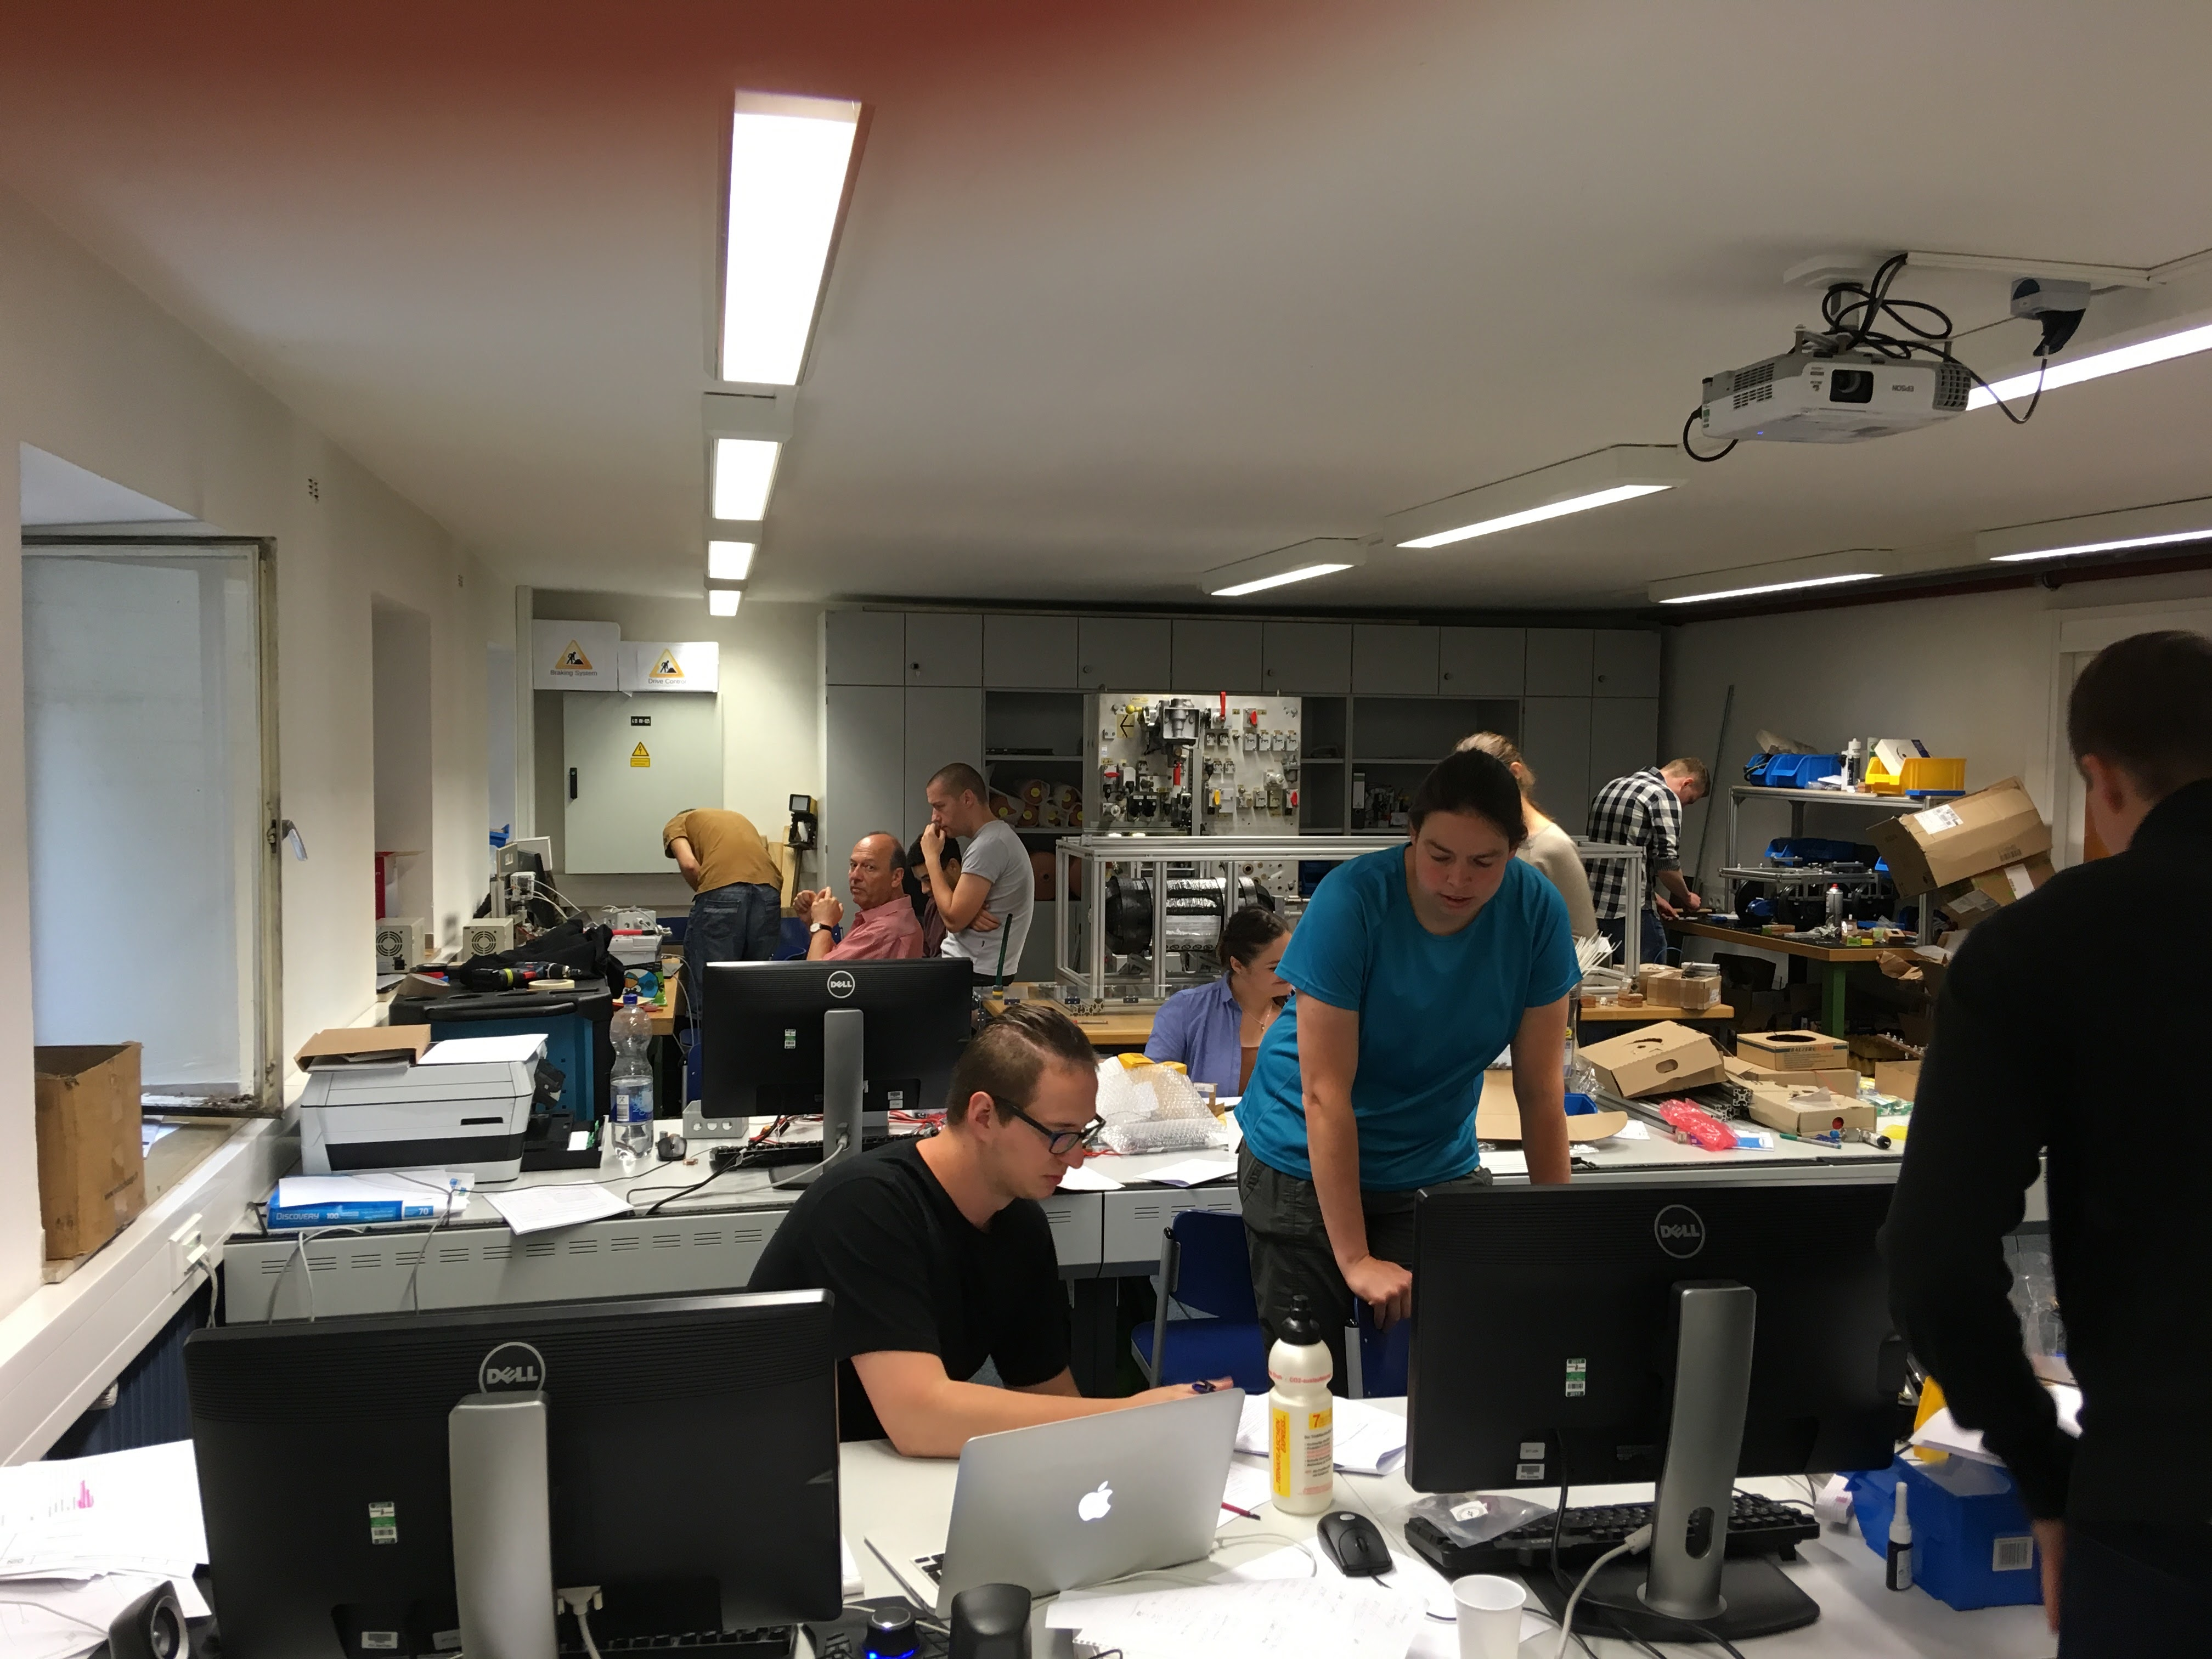
\includegraphics[width=1\textwidth]{IMG_0845}}
%			\only<2>{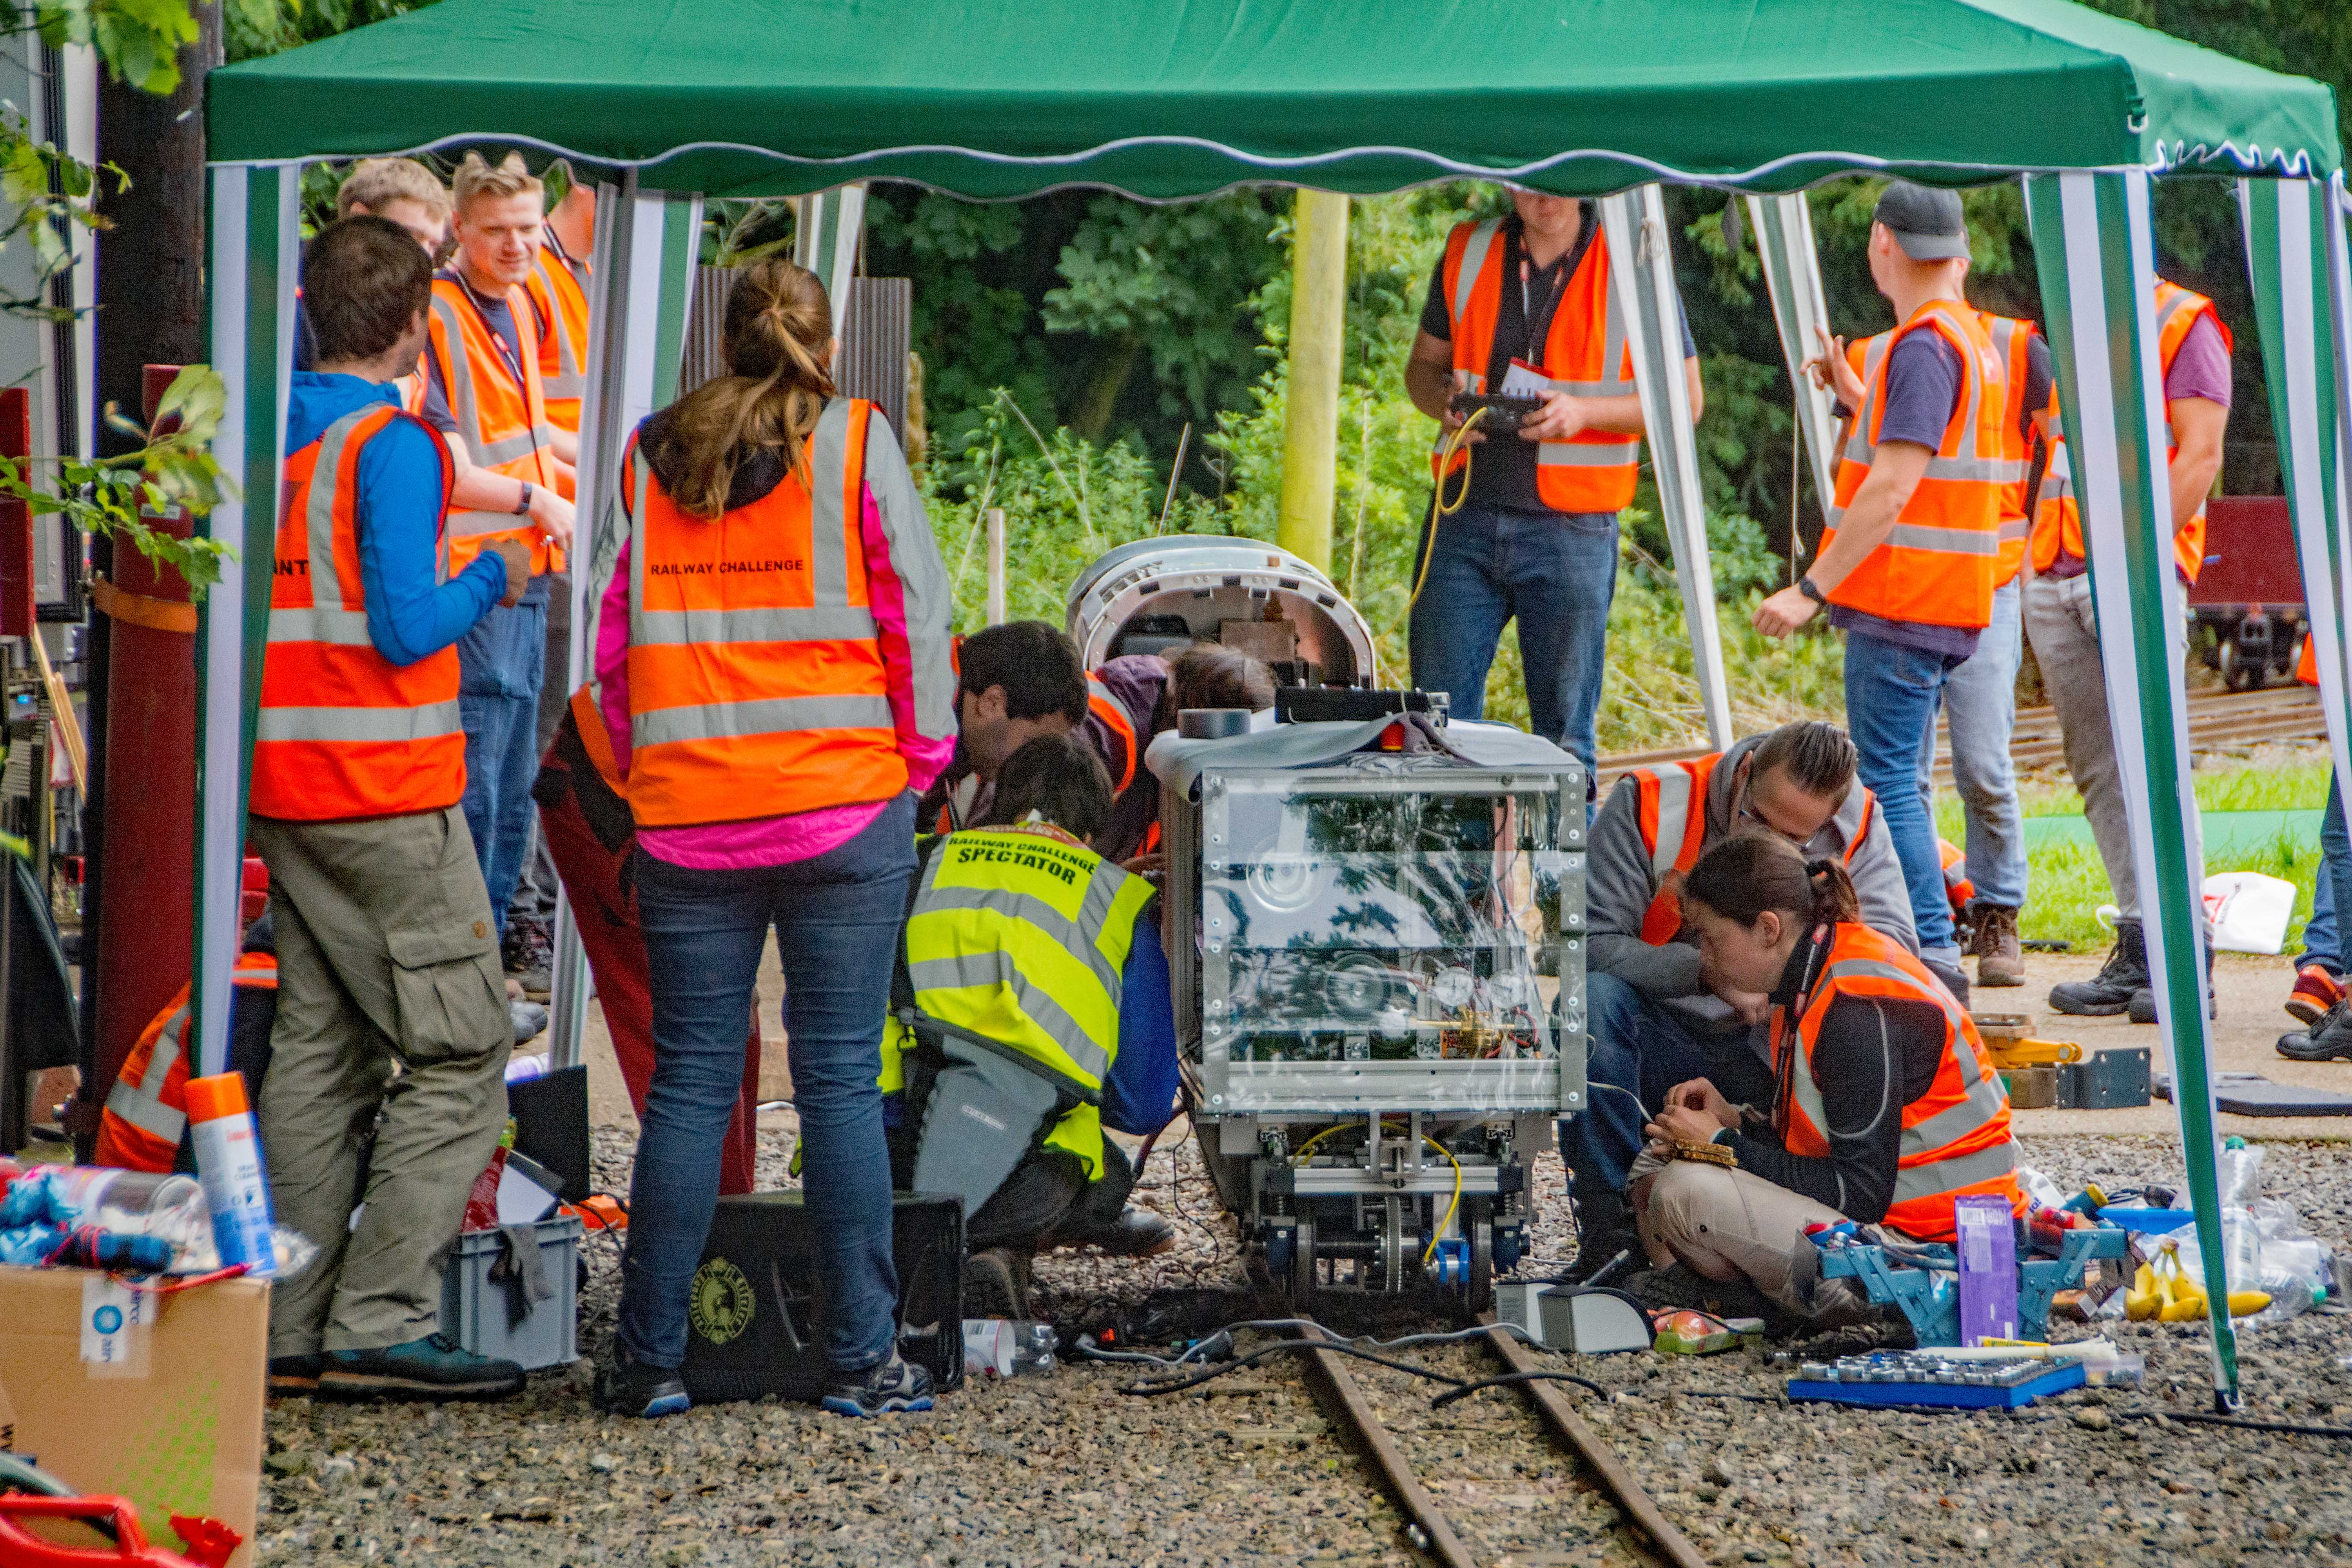
\includegraphics[width=1\textwidth]{DSC_1375}}
%			\only<3>{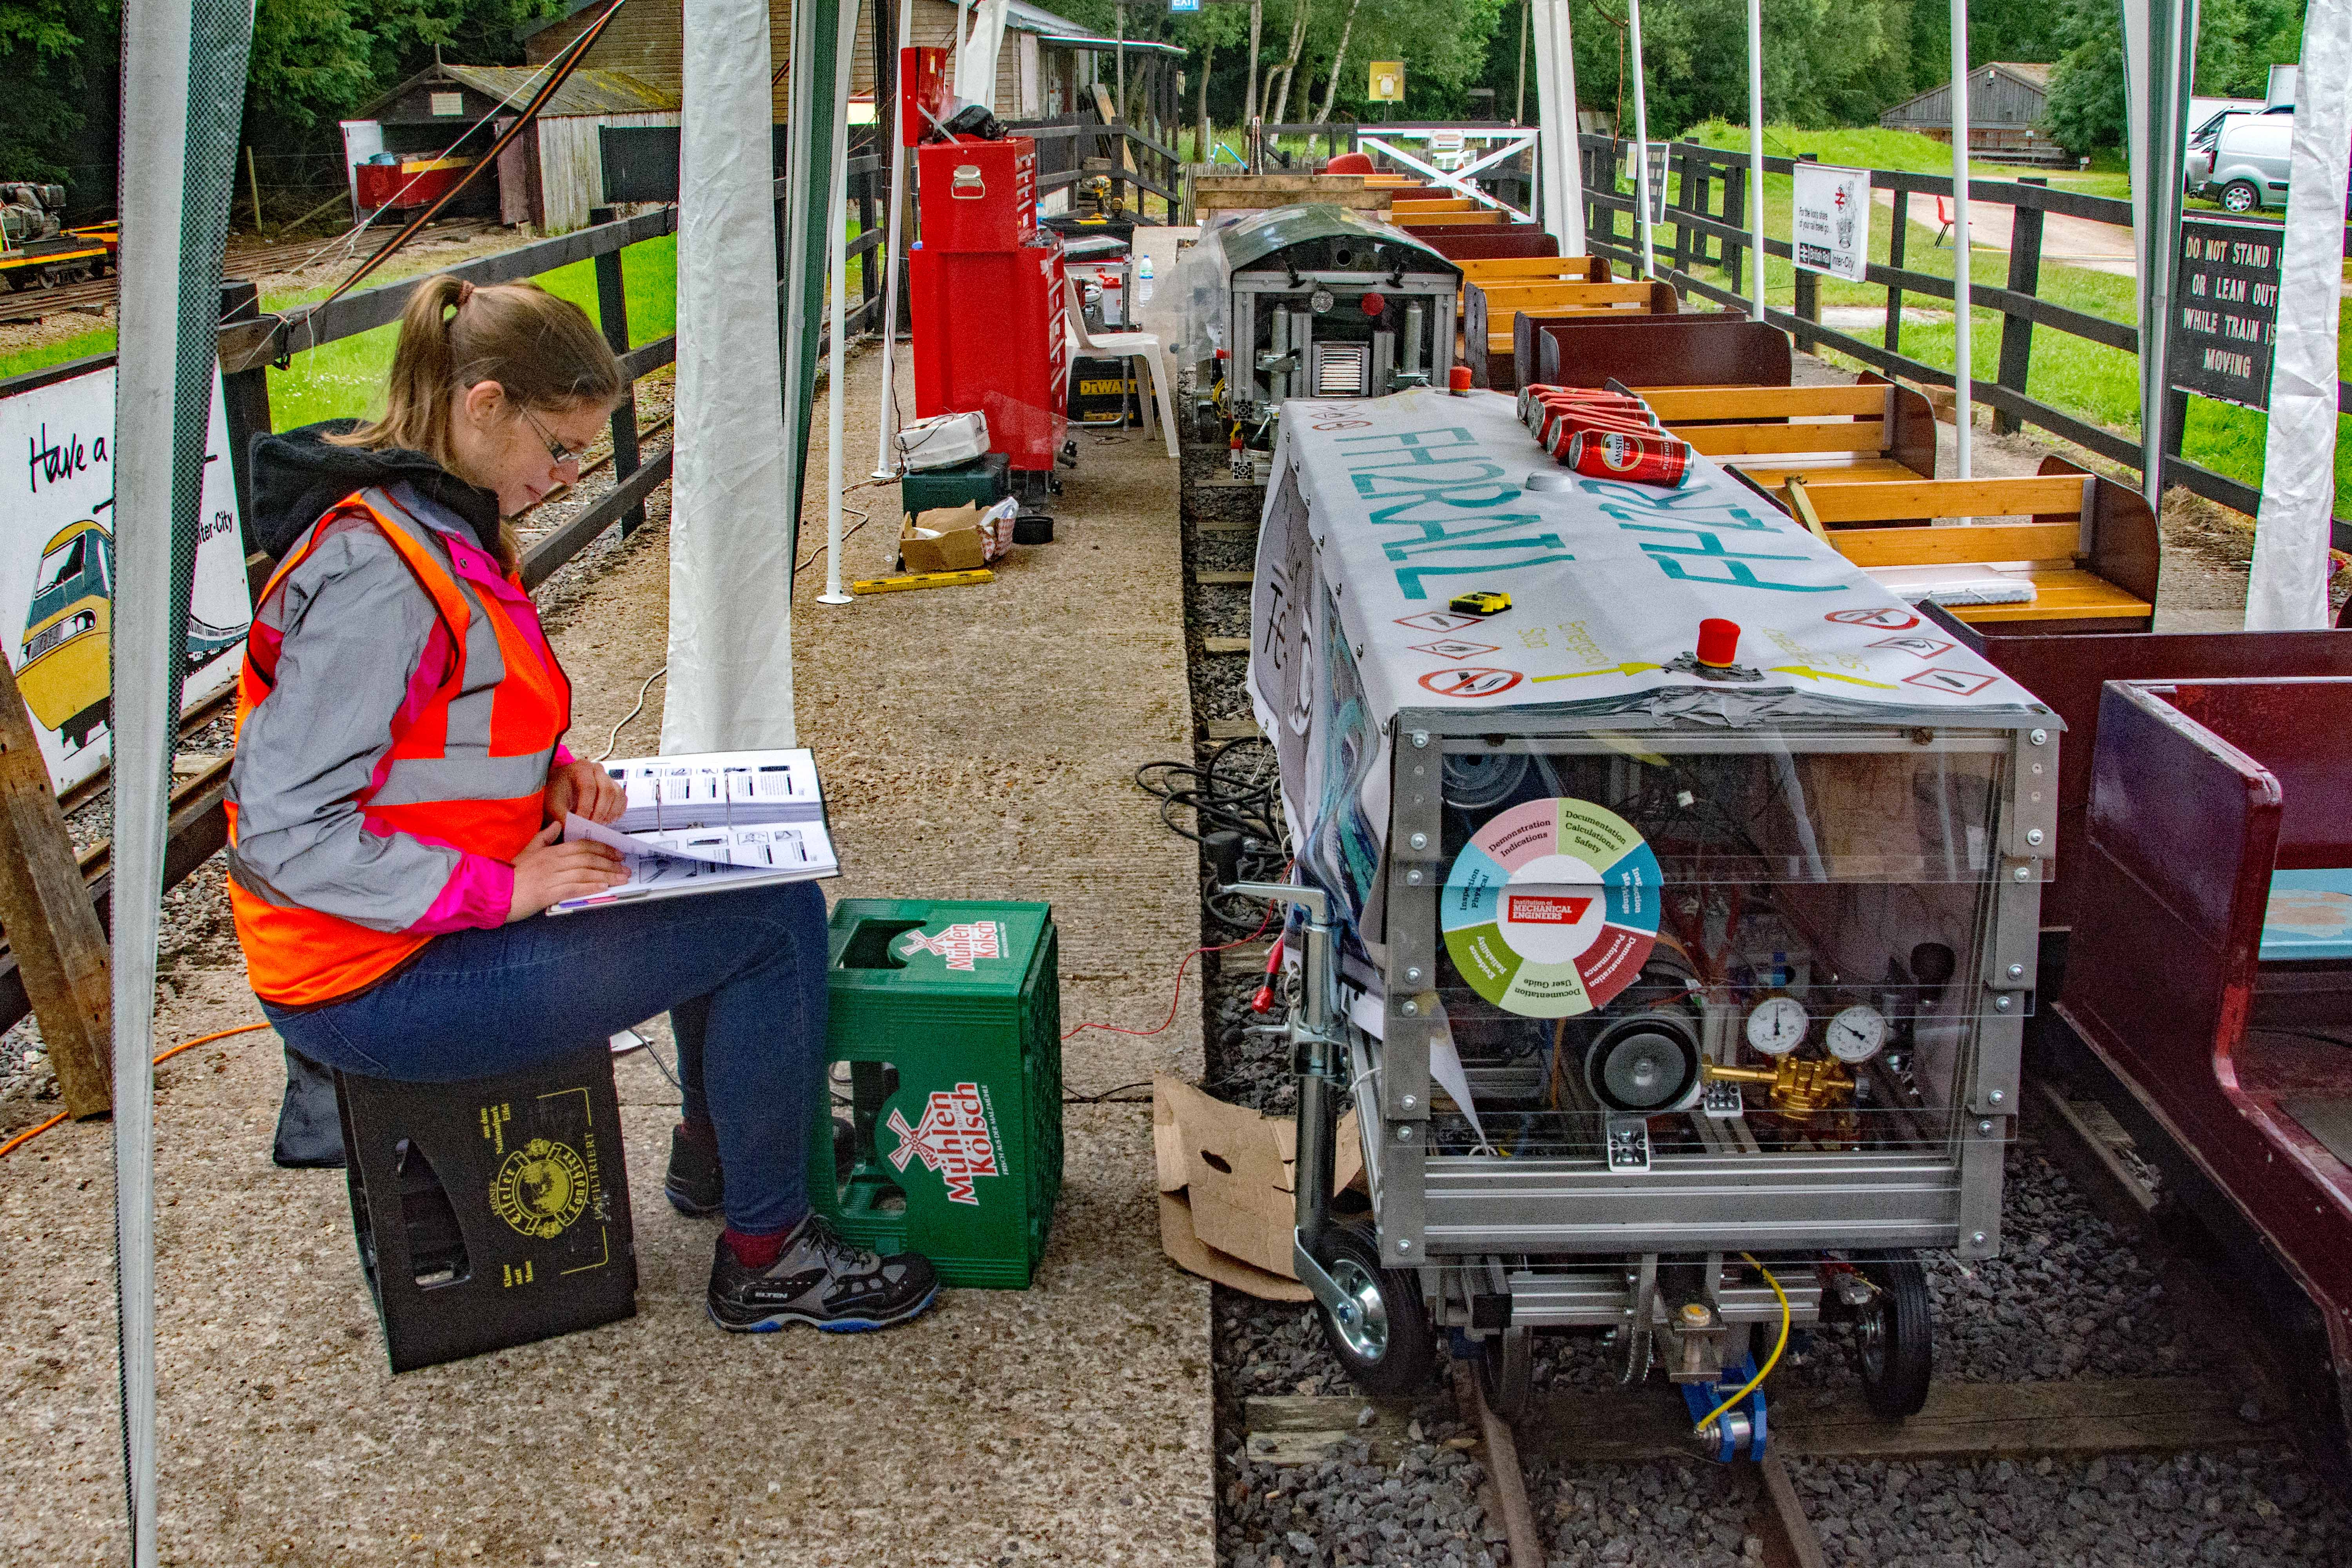
\includegraphics[width=1\textwidth]{DSC_1777}}
%			\only<4>{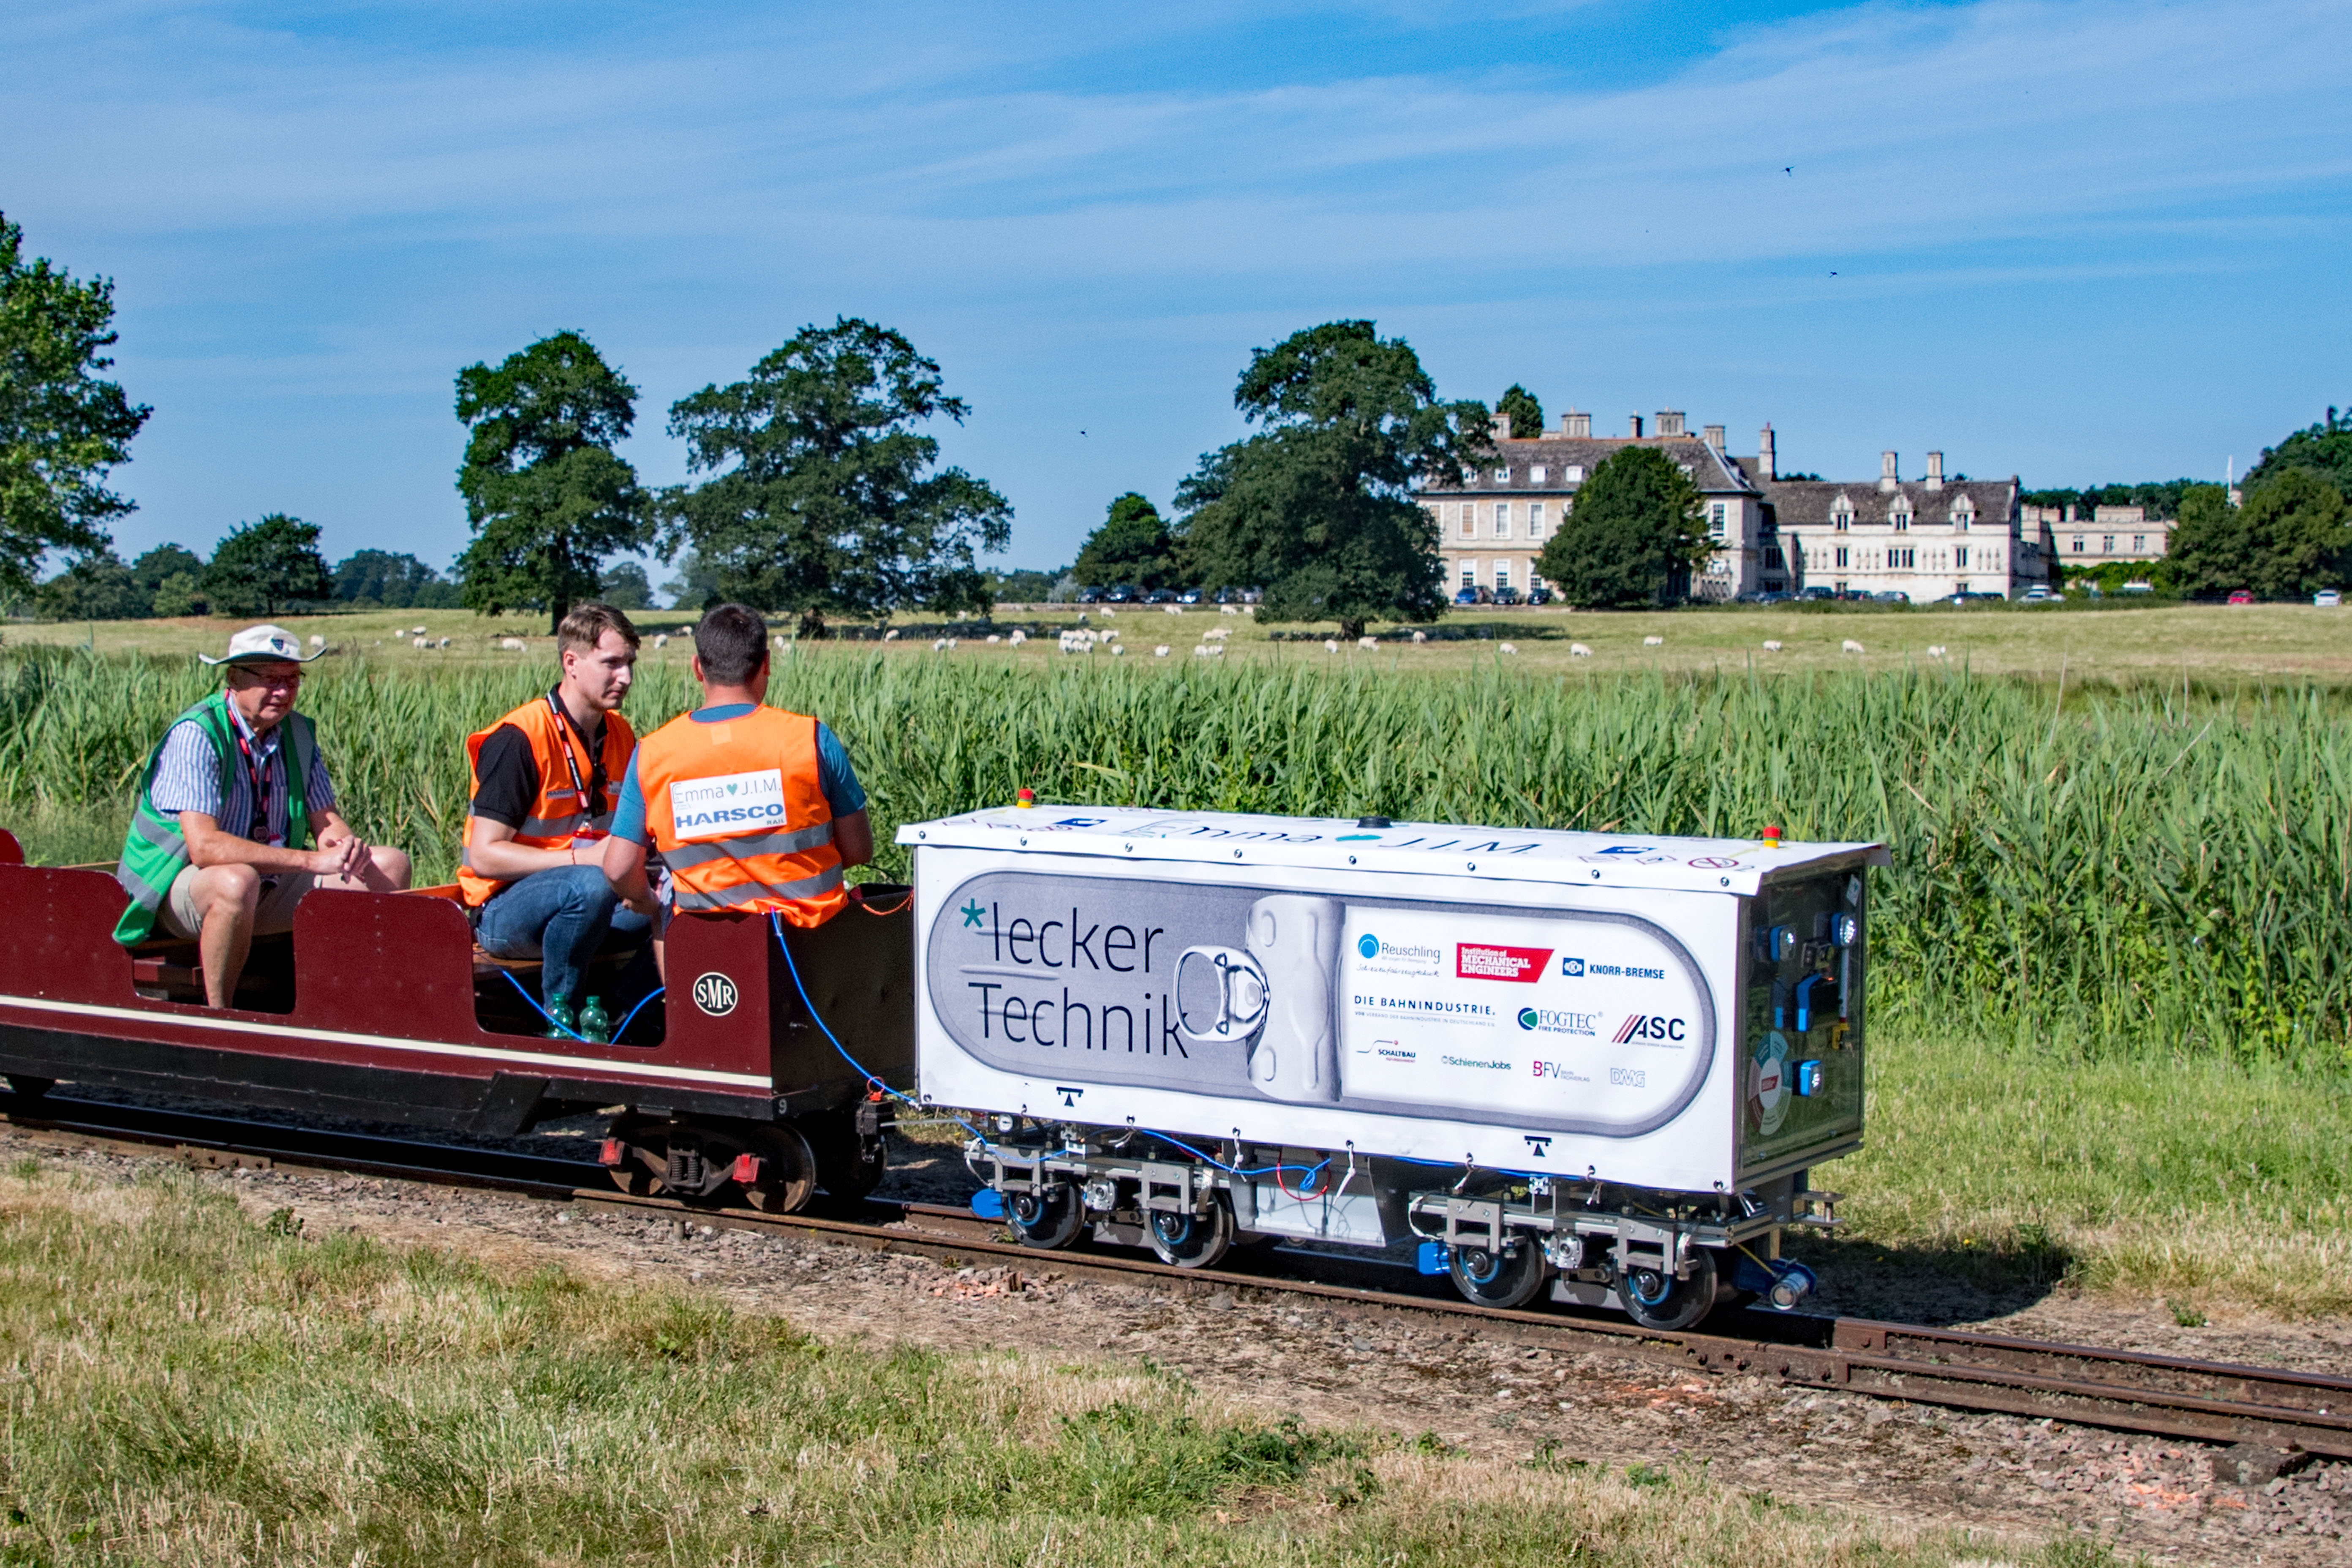
\includegraphics[width=1\textwidth]{EmmaCastle}}
%			\only<5->{\vspace{-.5cm}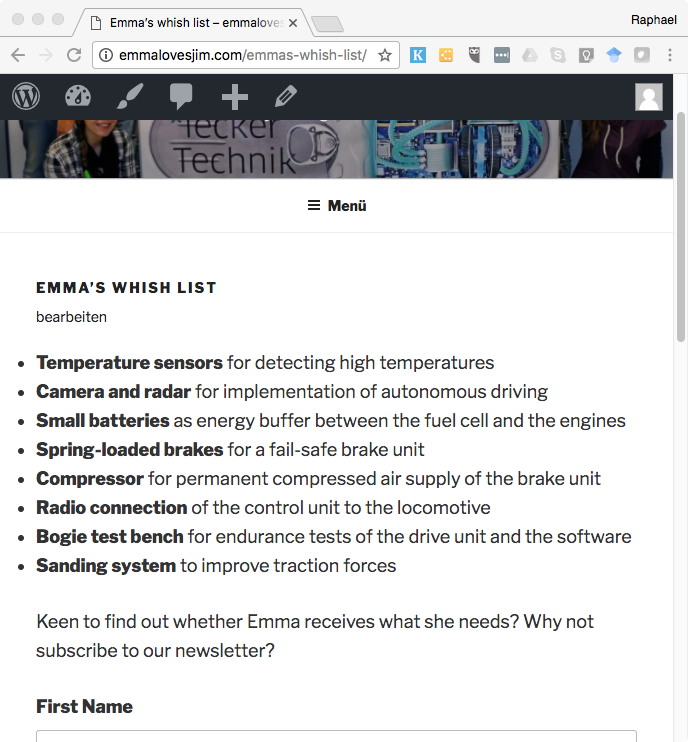
\includegraphics[width=.9\textwidth]{Whishlist}}
%        		\end{center}
%     \end{column}
% \end{columns}
%}

%{
%\usebackgroundtemplate{\includegraphics[width= \paperwidth]{EmmaCastlepale.jpg}}
%
%\frame{\frametitle{\color{white}Was kann die Railway Challenge der Bahnindustrie geben?}
%\framesubtitle{}
%\begin{itemize} %\color{white}
%\item Neues Bild von Studium und Beruf im Bereich Bahn
%\item Jugendliche Darstellung
%\item ``Du bist hier willkommen!''
%\item ``Du kannst etwas ausprobieren und etwas bewegen!''
%\item ``Coole Technik hier - und sinnvoll ist es auch!''
%\end{itemize}
%\vspace{-0.5cm}
%%\only<2>{\begin{center}
%%\Huge \textbf{\color{mint!75!black}
%%Dabei hilft Ihr Engagement!}
%%\end{center}}
%}
%}

%\usebackgroundtemplate{}

\section{Railway Challenge Continental Edition}

\frame{\frametitle{Warum eine ``eigene'' Railway Challenge?}
\framesubtitle{}
\begin{columns}[t] 
     \begin{column}[T]{6cm} 
     	\begin{itemize}
     		\item Vorbild Formula Student
		\begin{itemize}
			\item Gegr\"undet 1981 durch SAE
			\item Heute \"uber 500 Teams
			\item Erweiterung auf andere L\"ander seitens IMechE erw\"unscht
		\end{itemize}
		\item K\"onnen wir diese Erfolgsgeschichte wiederholen?
		\item Nicht nur in UK ist Eisenbahn attraktiv!
		\item Europ\"aische Pr\"agung durch Sponsoren etc.
		\item Strahlwirkung auf Jugendliche
     	\end{itemize}
     \end{column}
     	\begin{column}[T]{8cm} 
         	\begin{center}
            		\only<1>{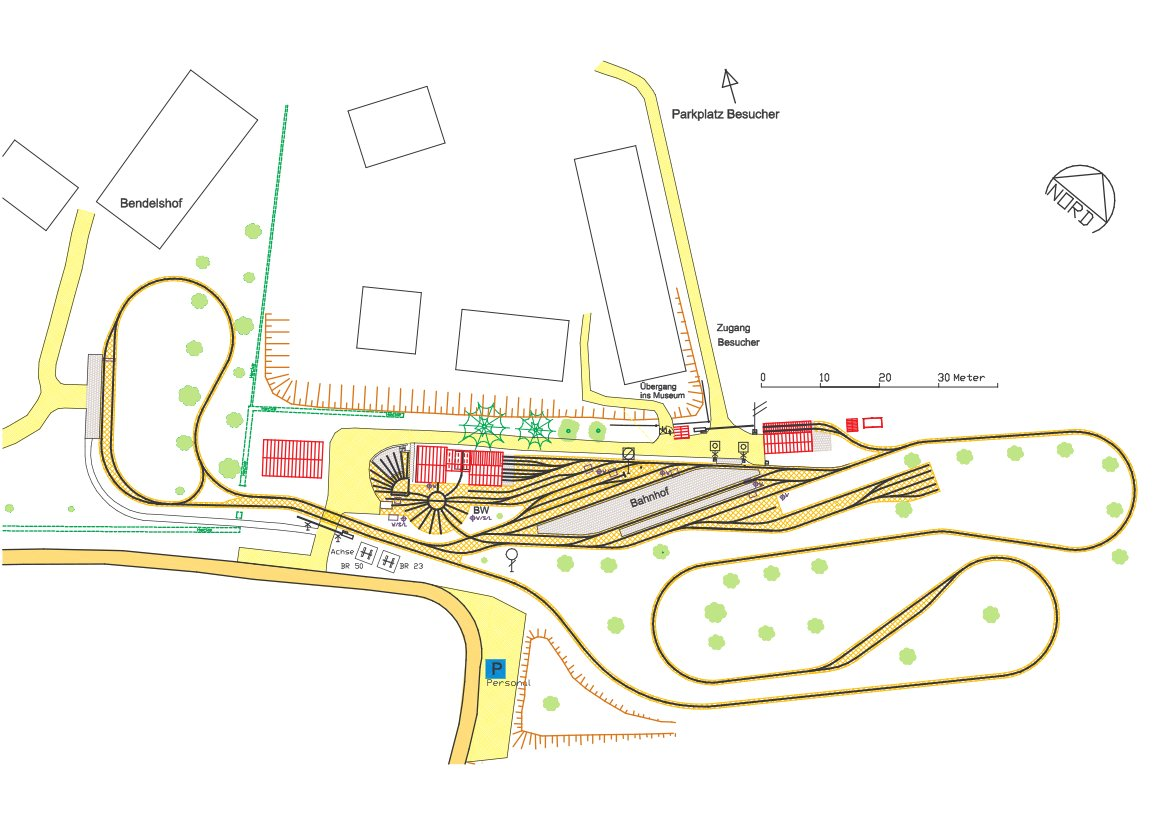
\includegraphics[width=0.9\textwidth]{lageplan}}
			\only<2>{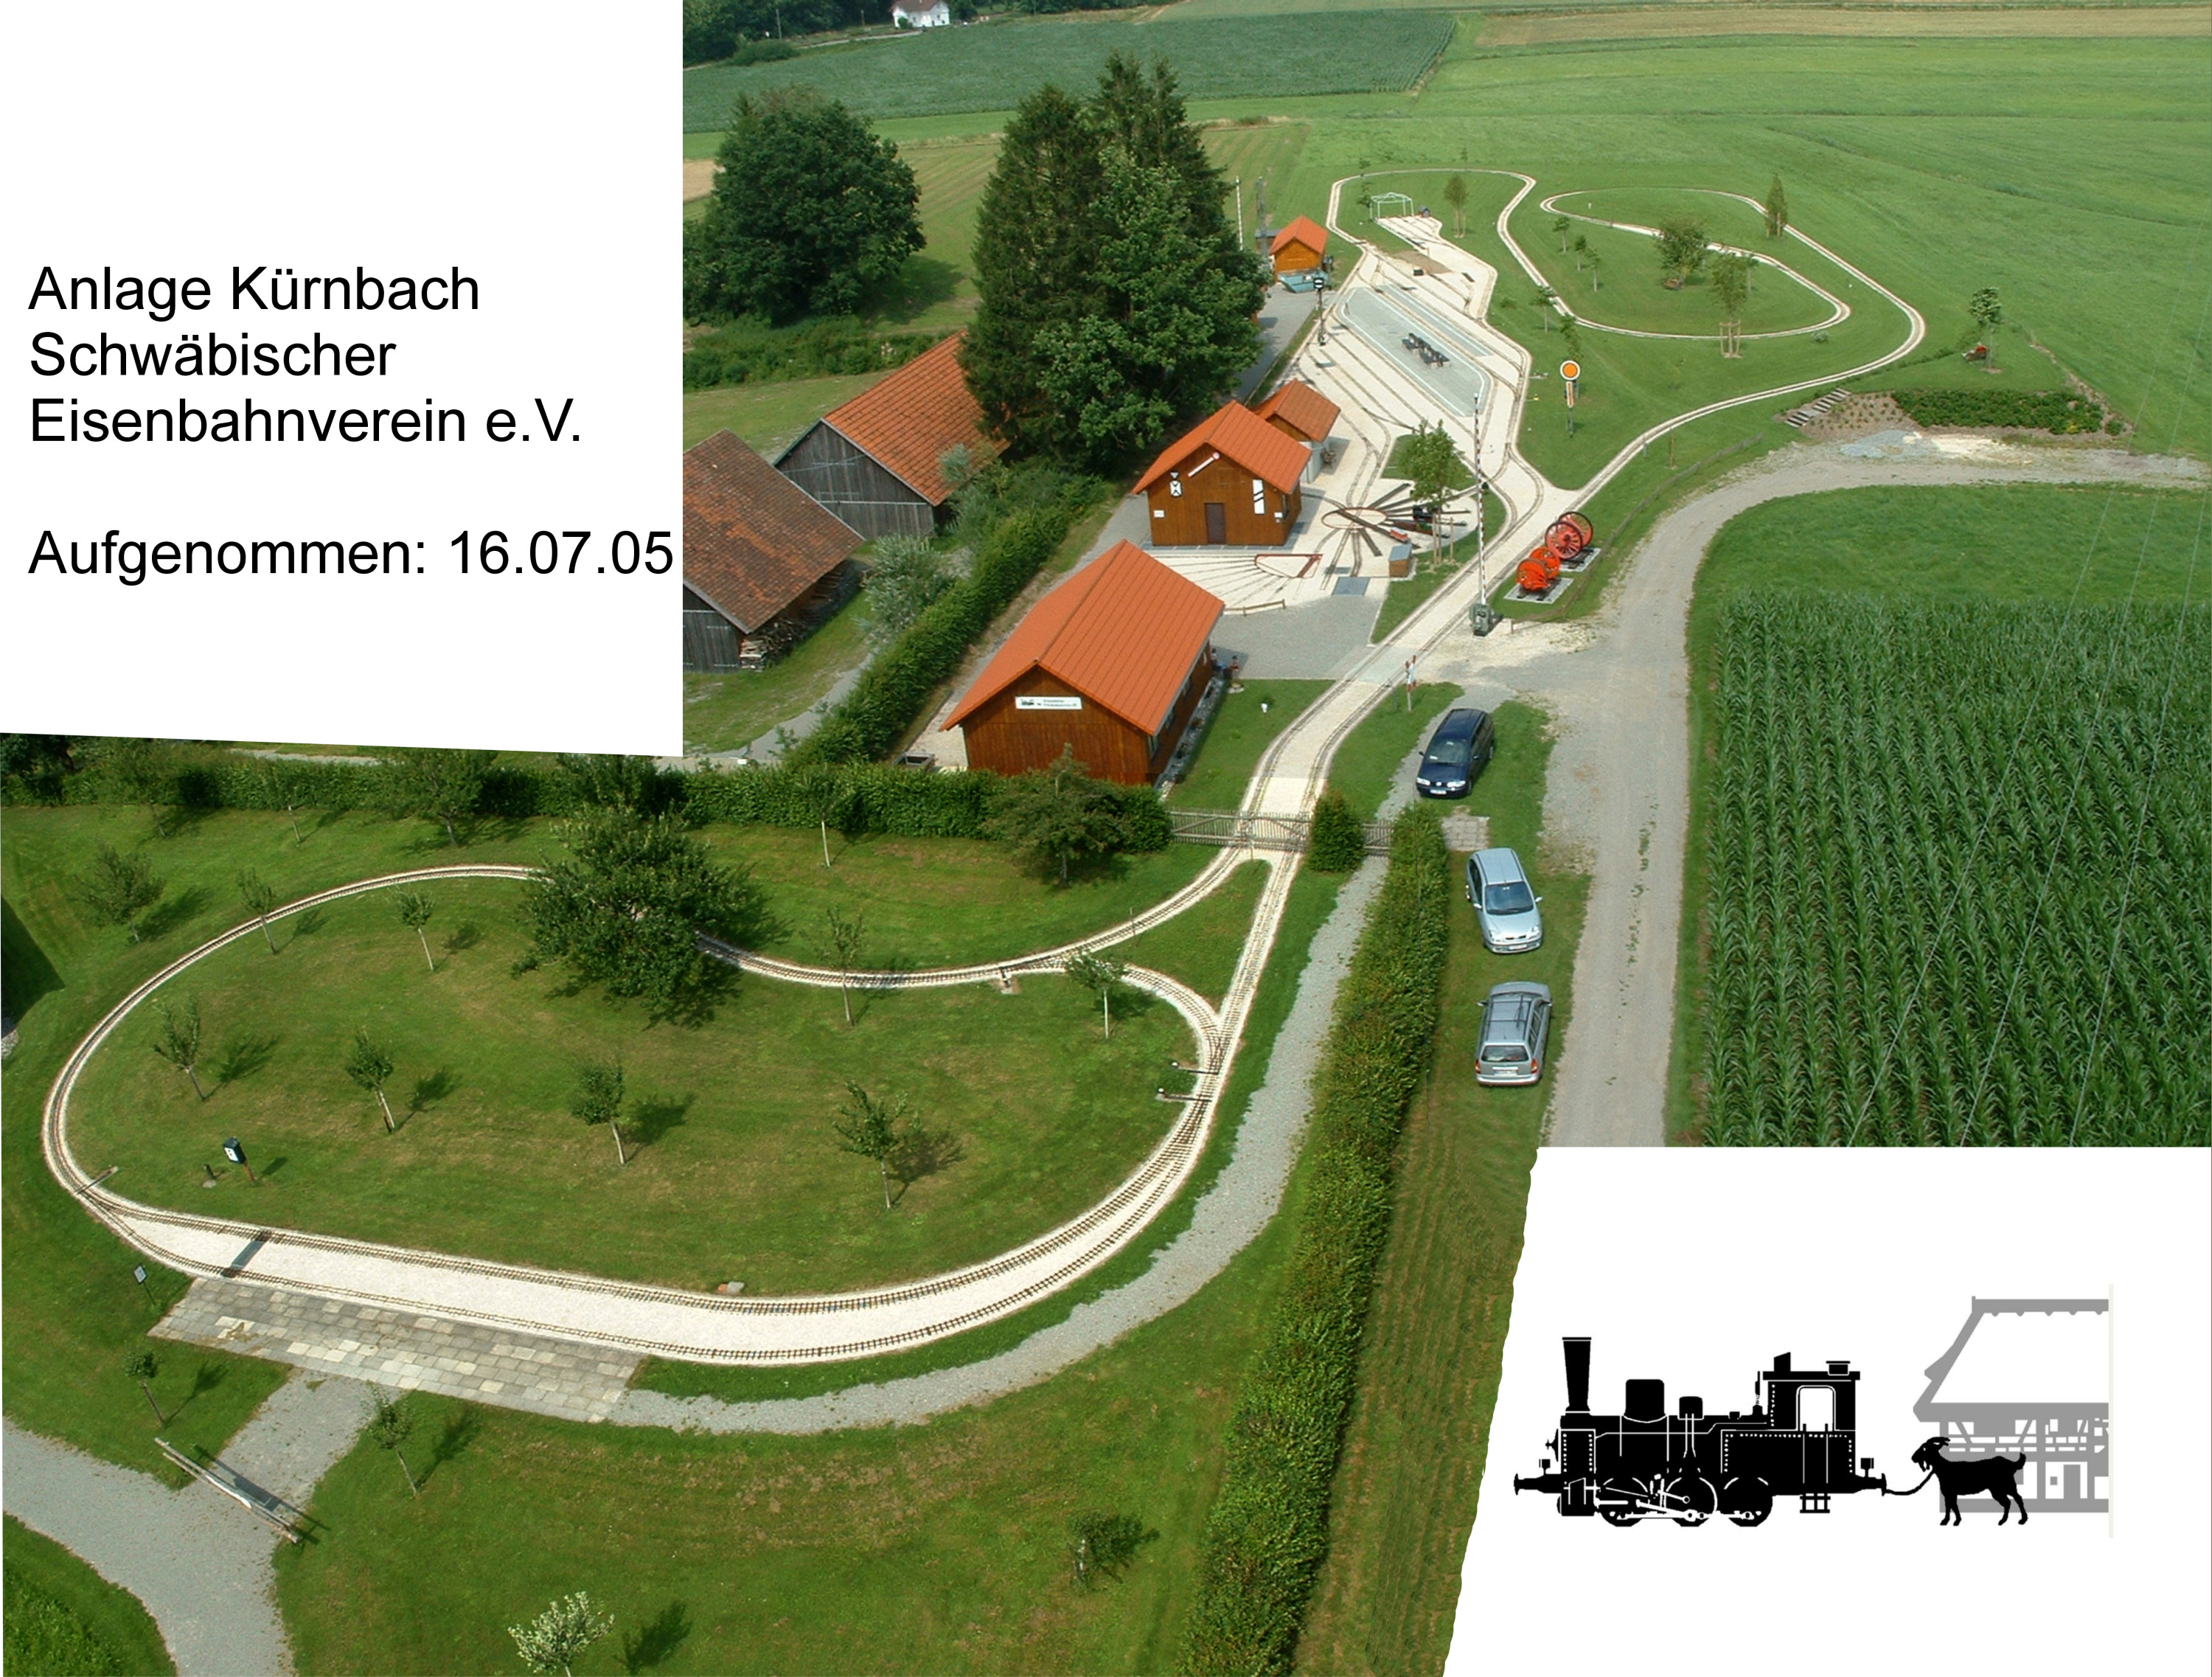
\includegraphics[width=0.9\textwidth]{luftbild}}
        		\end{center}
     \end{column}
 \end{columns}
}

\begin{frame}
\frametitle{Ablauf und Kostensch\"atzung}
\framesubtitle{}
\begin{itemize}
\item Strecke in Bad Schussenried (BW, nahe Bodensee): lokaler Verein hat sich bereit erklärt, uns zu beherbergen
\item Teams aus Europa
\item Termin des Events: Anfang Juni 2021, danach jährlich
\begin{itemize}
		\item Interessensbekundung der Teams Sommer 2020
		\item Registrierung Herbst 2020
		\end{itemize} 
\item Finanzbedarf: Schätzung ca. 20.000 EUR
\begin{itemize}
		\item Infrastruktur Wettkampfgelände (Zelt, Duschen, WC, Strom, ...) 10.000 EUR
    		\item Aufwandsentschädigung Parkbahn ~3.000 EUR
   		\item  Reisekosten Jury ~2.000 EUR
    		\item Siegprämien, Anschubfinanzierung (1-2 Teams nach England?) 5.000 EUR
    		\item Einnahmen von weiteren Sponsoren und aus Startgeldern		
		\end{itemize}
		\end{itemize}
%		\framebreak
%\item Personalbedarf:
%	\begin{itemize}
%		\item Eventmanagement, Registrierung, Weiterleiten der Dokumente, Koordination Helfer... ca. 6 Personenmonate
%    		\item Jury: 6 Mitglieder - Anwesenheit über das Wochenende (Fr-So) + Prüfen und Bewerten der Dokumente vorab. 	
%		\item Prominenter Head Judge
%    		\item Freiwillige der Parkbahn (z.B. im Bremswagen, Catering etc.)
%		\end{itemize}
\end{frame}
		
\begin{frame}
\frametitle{Unterst\"utzer derzeit}
Zugesichert derzeit von:
\begin{itemize}
		\item Verband der Bahnindustrie in Deutschland (Wettkampfb\"uro)
		\item Knorr-Bremse (personell und finanziell, Betrag offen)
		\item Westf\"alische Lokomotivfabrik Reuschling (personell, finanziell offen)
		\item Schaltbau Refurbishment (finanziell, Betrag offen)
		\item T\"UV S\"ud (personell, finanziell offen)
\end{itemize}
\end{frame}

\frame{\frametitle{Weitere Unterst\"utzung}
\framesubtitle{}
\begin{itemize}
\item Weitere unterst\"utzende Organisationen werden gesucht:
\begin{itemize}
	\item Als Sponsor f\"ur die Challenge allgemein (Levels werden festgelegt)
	\item Als Sponsor einzelner Wertungen, z.B. die ``MegaCorp Auto Stop Challenge''
	\item Produktsponsoring f\"ur die Teams
\end{itemize}
\item Stellen Sie ein Team - ihre Young Professionals (bis 2 Jahre nach Abschluss) und Azubis werden es Ihnen danken!
\item Unterst\"utzen Sie mit Personal, z.B. Judges
\end{itemize}
}


{
\usebackgroundtemplate{\includegraphics[width= 1\paperwidth]{Winners2019}}
\centering
\frame{\frametitle{Let's put awesome back into railways!}
\begin{tikzpicture}
 \path (0,0) -- (0cm,-7.3cm) node[rectangle, fill = white, opacity = 0.5, text opacity = 1] {Prof. Dr. Raphael Pfaff $\cdot$
			pfaff@fh-aachen.de $\cdot$
	%+49-151-70052454 $\cdot$
		www.emmalovesjim.com};
\end{tikzpicture}

}
\end{document}
